\documentclass[11pt]{article}


\usepackage{microtype}
\usepackage{graphicx}
\usepackage{wrapfig}
\usepackage{url}
\usepackage{color}
\usepackage{marvosym}
\usepackage{enumerate}
\usepackage{subfigure}
\usepackage{tikz}
\usepackage[fleqn]{amsmath}
\usepackage{amssymb}
\usepackage{hyperref}
\usepackage[many]{tcolorbox}
\usepackage{lipsum}
\usepackage{float}
\usepackage{trimclip}
\usepackage{listings}
\usepackage{environ}% http://ctan.org/pkg/environ
\usepackage{wasysym}
\usepackage{array}
\usepackage{bbm}
\usepackage{bm}
\usepackage{verbatim}

\oddsidemargin 0mm
\evensidemargin 5mm
\topmargin -20mm
\textheight 240mm
\textwidth 160mm



\newcommand{\vwi}{{\bf w}_i}
\newcommand{\vw}{{\bf w}}
\newcommand{\vx}{{\bf x}}
\newcommand{\vy}{{\bf y}}
\newcommand{\vxi}{{\bf x}_i}
\newcommand{\yi}{y_i}
\newcommand{\vxj}{{\bf x}_j}
\newcommand{\vxn}{{\bf x}_n}
\newcommand{\yj}{y_j}
\newcommand{\ai}{\alpha_i}
\newcommand{\aj}{\alpha_j}
\newcommand{\X}{{\bf X}}
\newcommand{\Y}{{\bf Y}}
\newcommand{\vz}{{\bf z}}
\newcommand{\msigma}{{\bf \Sigma}}
\newcommand{\vmu}{{\bf \mu}}
\newcommand{\vmuk}{{\bf \mu}_k}
\newcommand{\msigmak}{{\bf \Sigma}_k}
\newcommand{\vmuj}{{\bf \mu}_j}
\newcommand{\msigmaj}{{\bf \Sigma}_j}
\newcommand{\pij}{\pi_j}
\newcommand{\pik}{\pi_k}
\newcommand{\D}{\mathcal{D}}
\newcommand{\el}{\mathcal{L}}
\newcommand{\N}{\mathcal{N}}
\newcommand{\vxij}{{\bf x}_{ij}}
\newcommand{\vt}{{\bf t}}
\newcommand{\yh}{\hat{y}}
\newcommand{\code}[1]{{\footnotesize \tt #1}}
\newcommand{\alphai}{\alpha_i}
\newcommand{\defeq}{\overset{\text{def}}{=}}


\newcommand{\answer}[1]{{\bf\color{red}#1}}


%%%%%%%%%%%%%%%%%%%%%%%%%%%%%%%%%%%%%%%%%%%%%%%%%%%%%%%%%%%%%%%%%%%%%%%%%%%%%%%%
% Gradescope-friendly answer boxes

\bgroup
\def\arraystretch{1.5}
\newcolumntype{x}[1]{>{\centering\arraybackslash\hspace{0pt}}p{#1}}
\newcolumntype{z}[1]{>{\centering\arraybackslash}m{#1}}

%Arguments are 1 - height, 2 - box title
\newtcolorbox{textanswerbox}[2]{%
 width=\textwidth,colback=white,colframe=blue!30!black,floatplacement=H,height=#1,title=#2,clip lower=true,before upper={\parindent0em}}

 \newtcolorbox{eqanswerbox}[1]{%
 width=#1,colback=white,colframe=black,floatplacement=H,height=3em,sharp corners=all,clip lower=true,before upper={\parindent0em}}

 %Arguments are 1 - height, 2 - box title
 \NewEnviron{answertext}[2]{
        \noindent
        \marginbox*{0pt 10pt}{
        \clipbox{0pt 0pt 0pt 0pt}{
        \begin{textanswerbox}{#1}{#2}
        \BODY
        \end{textanswerbox}
        }
        }
}

%Arguments are 1 - height, 2 - box title, 3 - column definition
 \NewEnviron{answertable}[3]{
        \noindent
        \marginbox*{0pt 10pt}{
        \clipbox{0pt 0pt 0pt 0pt}{
        \begin{textanswerbox}{#1}{#2}
                \vspace{-0.5cm}
                        \begin{table}[H]
                        \centering
                        \begin{tabular}{#3}
                                \BODY
                        \end{tabular}
                        \end{table}
        \end{textanswerbox}
        }
        }
}

 %Arguments are 1 - height, 2 - box title, 3 - title, 4- equation label, 5 - equation box width
 \NewEnviron{answerequation}[5]{
        \noindent
        \marginbox*{0pt 10pt}{
        \clipbox{0pt 0pt 0pt 0pt}{
        \begin{textanswerbox}{#1}{#2}
                \vspace{-0.5cm}
                        \begin{table}[H]
                        \centering
                \renewcommand{\arraystretch}{0.5}% Tighter

                        \begin{tabular}{#3}
                                #4 =    &
                        \clipbox{0pt 0pt 0pt 0pt}{

                        \begin{eqanswerbox}{#5}
                                $\BODY$
                        \end{eqanswerbox}
                        } \\
                        \end{tabular}
                        \end{table}

        \end{textanswerbox}
        }
        }
}

 %Arguments are 1 - height, 2 - box title
 \NewEnviron{answerderivation}[2]{
        \noindent
        \marginbox*{0pt 10pt}{
        \clipbox{0pt 0pt 0pt 0pt}{
        \begin{textanswerbox}{#1}{#2}
        \BODY
        \end{textanswerbox}
        }
        }
}

\newcommand{\Checked}{{\LARGE \XBox}}%
\newcommand{\Unchecked}{{\LARGE \Square}}%
\newcommand{\TextRequired}{{\textbf{Place Answer Here}}}%
\newcommand{\EquationRequired}{\textbf{Type Equation Here}}%


\newcommand{\answertextheight}{5cm}
\newcommand{\answertableheight}{4cm}
\newcommand{\answerequationheight}{2.5cm}
\newcommand{\answerderivationheight}{14cm}

\newcounter{QuestionCounter}
\newcounter{SubQuestionCounter}[QuestionCounter]
\setcounter{SubQuestionCounter}{1}

\newcommand{\subquestiontitle}{Question \theQuestionCounter.\theSubQuestionCounter~}
\newcommand{\newquestion}{\stepcounter{QuestionCounter}\setcounter{SubQuestionCounter}{1}\newpage}
\newcommand{\newsubquestion}{\stepcounter{SubQuestionCounter}}

%%%%%%%%%%%%%%%%%%%%%%%%%%%%%%%%%%%%%%%%%%%%%%%%%%%%%%%%%%%%%%%%%%%%%%%%%%%%%%%%


\pagestyle{myheadings}
\markboth{Homework 2}{Fall 2019 CS 475 Machine Learning: Homework 2}


\title{CS 475 Machine Learning: Homework 2\\
Supervised Classifiers 2: Non-linear Classifiers\\
\Large{Due: Thursday October 10, 2019, 11:59pm}\\
100 Points Total \hspace{1cm} Version 1.1}
\author{}
\date{}

\begin{document}
\large
\maketitle
\thispagestyle{headings}

\vspace{-.5in}


\begin{answertext}{2cm}{}\centering
  Student name:  **** STUDENT NAME *****\\

\end{answertext}

{\bf Make sure to read from start to finish before beginning the assignment.}
\section{Programming (50 points)}
In this assignment, you will implement two regression models: regression trees and gradient boosted regression trees.
You will be using the same Python framework as before. Remember: \textbf{do not change the names of any of the files or command-line arguments that have already been provided.}

\subsection{Regression using trees}
You will implement two tree-based methods for regression: regression trees and gradient-boosted regression trees (GBRTs). Regression trees are a base object in GBRTs, so you should implement regression trees first, and then use that implementation to build the GBRT. You will be using these methods to predict the price of a house given 37 features describing the house. The data was extracted from here (\url{https://www.kaggle.com/c/house-prices-advanced-regression-techniques}) with some minor preprocessing.


\subsubsection{Regression Tree (20 points)}
\paragraph{Regression tree features:}

Regression trees, unlike decision trees, output a real value.  So we are given a
dataset of $n$ examples, $\{ (\boldsymbol{x}_i, y_i) \}^n_{i=1}$ where
$\boldsymbol{x}_i \in \mathbb{R}^D$ and $y_i \in \mathbb{R}$.  Since we are
doing \emph{regression}, we will not use log-likelihood or information gain to
decide which features to split on.  Instead, we will minimize the
\textbf{residual sum of squared error}, given the regression tree's prediction
function $f: \mathbb{R}^D \mapsto \mathbb{R}$,
\begin{equation}\label{eq:rss}
  \mathcal{E}(f) \defeq \sum_{i=1}^n (y_i - f(x_i))^2
\end{equation}

\noindent To support real-valued features, we will recursively split feature
dimensions $d$ based on feature thresholds $\theta$.  A schematic of such a tree
is given in figure \ref{fig:regression-tree}.

\begin{figure}\centering
    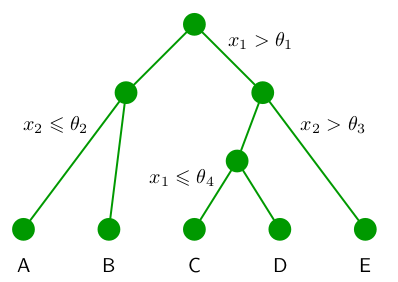
\includegraphics[width=90mm]{regression-tree.png}
    \caption{Illustration of regression tree (image credit to Chris Bishop's
      book). In this figure $x_1$ and $x_2$ are the first and second features of
      a specific example $x$.}
    \label{fig:regression-tree}
\end{figure}

\paragraph{Growing the tree:}
Much like the decision tree setting, each node in the decision tree partitions
the data of its parent node.  At each node, we will consider partitioning the
data at that node along each feature dimension.  Partitioning a dimension will
be done by a numeric threshold. Given the data at the node, $(X, \boldsymbol{y})$, a feature
dimension $d$, and a threshold $\theta$, we get two subsets of data indices.\footnote{$L$ of left of the threshold, $R$ for right of the threshold.}
%
\begin{align}\label{eq:split-set}
  L_{d,\theta}(X) &\defeq \{ i \mid X_{i,d} < \theta \} \\
  R_{d,\theta}(X) &\defeq \{ i \mid X_{i,d} \ge \theta \}
\end{align}

\noindent We will score a split according to the residual sum of squared errors
from the split-conditional mean\footnote{This is a reasonable heuristic because it
  is an upper bound: We know that we can achieve \emph{at least} as small as
  this residual value if we were to create leaf nodes on the next step (described later).}
%
\begin{equation}\label{eq:split-critera}
  s(L, R, \boldsymbol{y}) \defeq
  \sum_{i \in L } (y_i - \mu_{L})^2
  + \sum_{ i \in R } (y_i - \mu_{R})^2
\end{equation}
%
\noindent where $\mu_{L}$ and $\mu_{R}$ are the empirical mean of $y$ given the
respective set of points, $\mu_{L} \defeq \frac{1}{|L|} \sum_{i \in L} y_i$, and
similarly for $\mu_R$.  We will pick the split that minimizes
%
\begin{equation}
(d^*, \theta^*) = \underset{d \in \{1, \ldots, D \},\ {\color{blue}\theta \in \mathbb{R}}}{\mathrm{argmin}}\ s(L_{d,\theta}(X), R_{d,\theta}(X), \boldsymbol{y})
\end{equation}

\noindent In order to minimize this function with respect to real-valued
thresholds ${\color{blue}\theta \in \mathbb{R}}$, it turns out that we can limit the search to the following \emph{finite} set
\begin{equation}
\Theta_d(X) \defeq \{ X_{i,d} \mid i \in \{1, \ldots, n\}\}
\end{equation}

\noindent This gives is the following discrete optimization problem,
\begin{equation}\label{eq:opt-split}
(d^*, \theta^*) = \underset{d \in \{1, \ldots, D \},\ {\color{blue}\theta \in \Theta_d(X)} }{\mathrm{argmin}}\ s(L_{d,\theta}(X), R_{d,\theta}(X), \boldsymbol{y})
\end{equation}

\noindent Given the choice of the splitting criteria, $(d^*, \theta^*)$, we
create two children nodes with the appropriate $L$ and $R$ sets.  And,
recursively follow the same steps.

\paragraph{Base cases:}
Please use the following base cases for building decision trees:
\begin{enumerate}
\item There are $\le 1$ examples assigned to the node.
\item All features have zero variance in the examples assigned to the node
\item The path to the node has reached the maximum depth.\footnote{The depth of a node in a tree is the total length of the path between that node and the root of the tree. A tree of only a single root node has a depth of 0. In a decision tree, each node contains either a feature test or a value. Therefore, a tree of depth 0 can only contain a single node, which must just be a prediction value. A tree with a single feature test, which leads to a predicted value on both subsequent nodes, has depth 1 since each leaf is one step away from the root.}
\end{enumerate}


\paragraph{Leaf nodes: }
When we hit a base case, we will create a leaf node.  Each leaf node predicts a
constant value.  The choice for the constant value that optimizes the residual
sum of squares is the mean.  Therefore, leaves will predict the mean of its
$y$ data.


\paragraph{Remarks:}

\begin{itemize}
\item Feature dimension can be split multiple times.
\item Do not consider a split that results in empty sub-trees as this will result in an undefined residual sum of squared error.
\item A feature should not be considered for a split if the feature has no
  variance across the samples assigned to the node in order to avoid empty
  sub-trees (i.e., nodes with no samples assigned).
\end{itemize}


\paragraph{Speedup:}
If implemented naively, the split-selection optimization algorithm runs in time
$\mathcal{O}(N^2 D)$ because it recomputes the residual sum of squares (in time
$\mathcal{O}(N)$) for all possible features and thresholds (of which there are
$\mathcal{O}(D N)$ many). There are faster implementations that can run in
$\mathcal{O}(N D + N \log N)$.  However, we will leave such exploration up to
students.  We will give full credit for the slower implementation.

\newpage
\subsubsection{Gradient-Boosted Regression Tree (20 points)}
Gradient-Boosted Regression Trees (GBRT) use regression trees iteratively. At a high level, in each round of boosting, a regression tree is trained to predict the data points that were most difficult to accurately predict by trees in previous iterations of boosting (For more details see section 14.3-14.4 in Bishop: \url{https://www.microsoft.com/en-us/research/uploads/prod/2006/01/Bishop-Pattern-Recognition-and-Machine-Learning-2006.pdf}.) for reference on GBRTs.


\paragraph{GBRT Pseudocode: } The following pseudocode describes the GBRT algorithm. We assume that there are $N$ training examples, where a given example $i$ has label $y_i$ and feature vector $x_i$. $M$ is the model hyper-parameter (n-estimators) representing the number boosting (training) iterations. $0 < \lambda \le 1$ is the hyper-parameter (regularization-parameter) used to regularize the regression function.\\
\begin{enumerate}
\item Initialize the GBRT model ($F_0(x_i)$) to an the mean of your labels:\\
$F_0(x_i)=\frac{1}{N}\sum_{i=1}^N y_i$
\item For iteration $m = 1$ to $M$:
\begin{enumerate}[(a)]
\item Calculate the residuals given the current GBRT model. Specifically, use
  $F_{m-1}$ to make predictions on each of the training examples
  ($F_{m-1}(x_i)$). Then, using the predictions, calculate the residuals
  according to:
 \begin{equation}
   g_i^{(m)} = y_i - F_{m-1}(x_i) \quad\text{for } i = 1 \ldots N
 \end{equation}
\item Fit a regression tree $h_m(x)$ to the training data $\{ (x_i, g^{(m)}_i) \}$
  (Use your implementation from section 1.1.2. Make sure to use the max depth
  parameter, which is give as a command-line option.)
\item Update the model: $F_m(x) = F_{m-1}(x) + \lambda h_m(x)$
\end{enumerate}
\item Return $F_M(X)$
\end{enumerate}

\newpage
\subsubsection{Implementation Details}
The two algorithms you implement in this assignment will be selected using arguments passed to the command-line argument {\tt --algorithm}. The arguments are {\tt regression-tree} and {\tt gradient-boosted-regression-tree}.

Your code must correctly implement the behavior described by the following
command-line options, which are passed in as arguments to the constructor of
your implementation in {\tt models.py}.
\begin{itemize}
\item {\tt --max-depth} The maximum depth a tree can be grown to. The default is
  3. This is used for both {\tt regression-tree} and
  \texttt{gradient-boosted-regression-tree}.
\item {\tt --n-estimators} The number of number of iterations (or equivalently
  the number of regression trees) used for {\tt
    gradient-boosted-regression-tree}. By default, this value is 100.
\item {\tt --regularization-parameter} The regularization parameter used by
  \\{\tt gradient-boosted-regression-tree}. By default, this value is 0.1.
\end{itemize}


\subsubsection{Examples}
As an example, the following trains a regression tree on the training data given
in a file {\tt train.txt} that we parse and load for you:
\begin{footnotesize}
\begin{verbatim}
python3 main.py --mode train --algorithm regression-tree --model-file regression.tree.model \
                --train-data train.txt
\end{verbatim}
\end{footnotesize}

\noindent To run the trained model on development data:
\begin{footnotesize}
\begin{verbatim}
python3 main.py --mode test --model-file regression.tree.model --test-data dev.txt \
                --predictions-file dev.predictions
\end{verbatim}
\end{footnotesize}

\noindent We provide the script {\tt compute\_mean\_square\_error.py} to
evaluate the root mean squared error of your model's predictions:
\begin{footnotesize}
\begin{verbatim}
python3 compute_root_mean_square_error.py dev.txt dev.predictions
\end{verbatim}
\end{footnotesize}

\subsubsection{Jupyter Notebook (10 points)}
We have provided a Jupyter Notebook ({\tt Regression-Experiments.ipynb}) containing several experiments that explore differences between regression trees and GBRTs, as well as the effects of hyper-parameter choice on the two models. After you have finished your implementations of regression trees and GBRTs, run the entire notebook and complete the prompt at the bottom of the notebook. Then create a PDF file containing the notebook after it has been run so we can see all of your output.

\newpage
\section{Analytical (50 points)}

\paragraph{Instructions}
We have provided this \LaTeX{} document for turning this homework. We give you
one or more boxes to answer each question.  The question to answer for each box
will be noted in the title of the box. {\bf Do not type anything outside the
  boxes. Leave the rest of the document unchanged.  There is a box for your name
  on the first page of this document. }

For written answers, replace the \lstinline{\TextRequired} (\TextRequired)
command with your answer. For the following example \textit{\subquestiontitle},
you would place your answer where \lstinline{\TextRequired} (\TextRequired) is
located,

\begin{answertext}{2.1cm}{}
\TextRequired
\end{answertext}
\newsubquestion
Do not change the height or title of the box. If your text goes beyond the box boundary, it will be cut off.  We have given sufficient space for each answer, so please condense your answer if it overflows. The height of the box is an upper bound on the amount of text required to answer the question - many answers can be answered in a fraction of the space.  Do not add text outside of the boxes. We will not read it.

%For True/False or Multiple Choice questions, place your answers within the defined table.  To mark the box(es) corresponding to your answers, replace \lstinline{\Unchecked} (\Unchecked) commands with the \lstinline{\Checked} (\Checked) command. Do not make any other changes to the table. For example, in \textit{\subquestiontitle},

%\begin{answertable}{2.5cm}{}{x{0.5cm}p{5cm}}
%\Checked &  Logistic Regression \\
%\Unchecked & Perceptron \\
%\end{answertable}

\newsubquestion
%For answers that require a single equation, we will provide a specific type of box, such as in the following example \textit{\subquestiontitle}.  Please type the equation where  \lstinline{\EquationRequired} (\EquationRequired) without adding any \$ signs or \lstinline{\equation} commands.  Do not put any additional text in this field.

%\begin{answerequation}{\answerequationheight}{}{z{1cm}z{12cm}}{\textbf{w}}{12cm}
%\EquationRequired
%\end{answerequation}
\newsubquestion
For answers that require multiple equations, such as a derivation, place all equations within the specified box.   You may include text short explanations if you wish (as shown in \textit{\subquestiontitle}).  You can put the equations in any format you like (e.g. within \$ or \$\$, the \lstinline{\equation} environment, the \lstinline{\align} environment) as long as they stay within the box.

\begin{answerderivation}{3.25cm}{}
\begin{align*}
x + 2  && \text{x is a real number} \\
&&\text{the following equation uses the variable } y \\
y+3
\end{align*}
\end{answerderivation}
\newsubquestion

\begin{itemize}
\item \textbf{Do not change any formatting in this document, or we may be unable
  to grade your work. This includes, but is not limited to, the height of
  textboxes, font sizes, and the spacing of text and tables.  Additionally, do
  not add text outside of the answer boxes. Entering your answers are the only
  changes allowed. }
\item \textbf{We strongly recommend you review your answers in the generated PDF to
  ensure they appear correct. We will grade what appears in the answer boxes in
  the submitted PDF, NOT the original latex file.}
\end{itemize}


\newquestion
\section*{\arabic{QuestionCounter}) Decision Trees (9 points)} {
Consider the classification task where you want to predict $y$ given $x_1, x_2,
x_3, x_4, x_5$.
\begin{center}
\begin{tabular}{ ccccc|c }
 $x_1$ & $x_2$ & $x_3$ & $x_4$ & $x_5$ & $y$ \\\cline{1-5}
 \hline
 1 & 0 & 0 & 0 & 1 & 1 \\
 1 & 0 & 1 & 0 & 1 & 1 \\
 0 & 1 & 0 & 1 & 1 & 1 \\
 0 & 0 & 0 & 1 & 1 & 0 \\
 1 & 1 & 1 & 0 & 1 & 0 \\
 1 & 0 & 1 & 1 & 1 & 0 \\
 1 & 0 & 0 & 1 & 1 & 0 \\
 0 & 1 & 0 & 0 & 1 & 0 \\
\end{tabular}
\end{center}

\begin{enumerate}[{(1)}]

\item Construct a decision tree based on the above training examples following
  the algorithm we specified in class using the information gain criterion and a
  maximum depth of 2.  As an additional base case, stop expanding if all
  training examples have the same label. You may use each feature at most once
  along any path from the root to a leaf.

  Using the decision tree schematic below, specify the correct feature number
  for internal nodes A, B, and C.  For each nodes D, E, F, and G, specify the
  correct label.  Put answers in the pre-formatted table by the ``?''  with the
  correct feature or label.


\parbox{9.25cm}{
    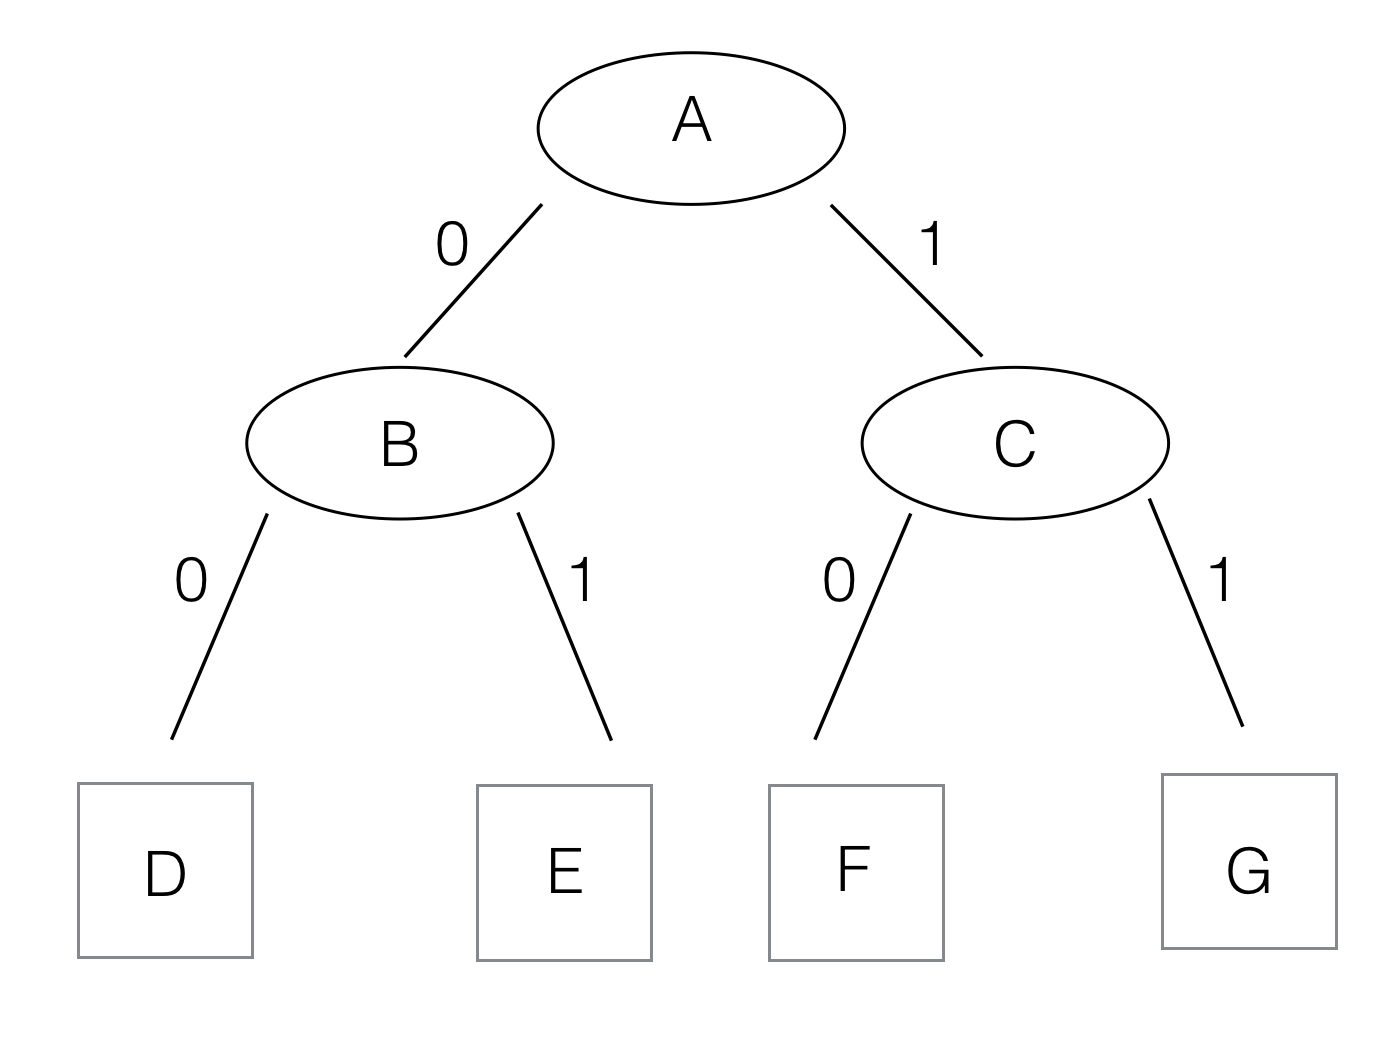
\includegraphics[width=90mm]{plot.png}
}
\begin{minipage}{5.5cm}
\begin{answertable}{6.5cm}{}{rc}
\text{Node} & Id or label  \\ \hline
A= & $x_4$ \\
B= & $x_2$ \\
C= & $x_2$ \\
D= & 1 \\
E= & 0 \\
F= & 0 \\
G= & 1 \\
\end{answertable}
\end{minipage}

\newpage
\item Apply the decision tree learned in part 1 of this question to classify the
  following new data points.  Replace the ``?'' in the table below with the
  classifier's prediction.

\begin{answertable}{3.5cm}{}{ccccc|c}
$x_1$ & $x_2$ & $x_3$ & $x_4$ & $x_5$ & $y$ \\ \hline
0 & 1 & 1 & 1 & 1 & 1 \\
1 & 1 & 0 & 1 & 1 & 1 \\
1 & 1 & 0 & 0 & 1 & 0 \\
\end{answertable}


\item For the training dataset in part 1, can any of the methods listed in the
  table below obtain a \emph{training accuracy} of 100\% using only the features given?
  Answer below by replacing the ``?'' with ``Y'' or ``N''.

\begin{answertable}{7cm}{}{l|c}
Method & $Y/N$ \\ \hline
Decision tree of depth 1 & $N$ \\
Decision tree of unlimited depth & $Y$ \\
Logistic regression & $N$ \\
Perceptron & $N$ \\
Linear Kernel SVM & $N$ \\
Quadratic Kernel SVM & $Y$ \\
\textsc{AdaBoost} with decision stumps & $Y$
\end{answertable}


\end{enumerate}

}


\newquestion
\section*{\arabic{QuestionCounter}) Kernels (10 points) } {

\begin{enumerate}[(1)]

\item Give $\mathcal{O}(\cdot)$ bounds for the different cases below in terms of
  the following quantities:%
  \begin{center}
  \begin{tabular}{ll}
    number of training examples & $n$ \\
    number of support vectors   & $s$ \\
    feature dimensionality      & $d$ \\
    kernel evaluation time      & $k$ \\
    size of an example          & $e$
  \end{tabular}
  \end{center}

  Suppose in each case below that we are predicting labels for $m$ test examples

\begin{answertable}{3.5cm}{}{l|l}
 The running time for a kernel SVM & $\mathcal{O}( ?  )$ \\
 The running time for a primal SVM & $\mathcal{O}( ?  )$ \\
 The space complexity for a kernel SVM & $\mathcal{O}( ? )$ \\
 The space complexity for a primal SVM & $\mathcal{O}( ? )$ \\
\end{answertable}


\item Suppose I trained a kernel SVM using a Gaussian kernel: $K(x, x') \defeq
  \exp\left( \frac{-||x - x'||^2}{ 2\sigma^2 } \right)$, where $\sigma$ is a
  positive scalar.  If my training set accuracy is very low, should I increase
  or decrease $\sigma$? Why?

  \begin{answertext}{3.5cm}{}

  \end{answertext}

\end{enumerate}

}



\newquestion
\section*{\arabic{QuestionCounter}) \textsc{AdaBoost} (10 points) } {

Assume a one-dimensional dataset with $x = \langle -1, 0, 1 \rangle$ and $y =
\langle -1, +1, -1 \rangle$.  Consider three weak classifiers:
\begin{align*}
  h_1(x) = \begin{cases}
    1  & \text{if } x > \frac{1}{2} \\
    -1 & \text{otherwise}
  \end{cases},
  \quad\quad
  h_2(x) = \begin{cases}
    1  & \text{if } x > - \frac{1}{2} \\
    -1 & \text{otherwise}
  \end{cases},
  \quad\quad
  h_3(x) = 1.
\end{align*}

\begin{enumerate}[(1)]
  \newsubquestion


\item Show your work for the first $2$ iterations of \textsc{AdaBoost}. You must use the
  method from the lecture slides to get full credit.\footnote{The method from
    class is equivalent to the algorithm in Figure 1 of
    \url{https://cseweb.ucsd.edu/~yfreund/papers/IntroToBoosting.pdf}} In the
  table below, replace the ``?'' in the table below with the value of the
  quantity at iteration $t$.  $h_t \in \{1,2,3\}$, weak learner's weight in the
  ensemble, $\alpha_t$, error rate, $\varepsilon_t$.  Additionally, give the
  distribution over example at iteration $t$, $D_{t}(1), D_{t}(2), D_{t}(3)$.
  Use $\log$ with base $e$ in your calculations.

\begin{answertable}{7cm}{}{c|ccc|ccc}
$t$ & $h_t$ & $\alpha_t$ & $\varepsilon_t$ & $D_{t}(1)$ & $D_{t}(2)$ & $D_{t}(3)$ \\ \hline
1 & 2 & 0.3466 & $\frac13$ & $\frac13$ & $\frac13$ & $\frac13$ \\
2 & 2 & 0 & 0.5 & $\frac14$ & $\frac14$ & $\frac12$ \\
\end{answertable}


\item After running \textsc{AdaBoost} for 10 iterations, what is the error rate of the ensemble?

\begin{answertext}{1cm}{}
  $\frac13$, it does not change after the first iteration
\end{answertext}

\newpage
\newsubquestion
\item In general, getting near-perfect training accuracy in machine learning
  leads to overfitting.  However, \textsc{AdaBoost} can get perfect training accuracy
  within overfitting.  Give a brief justification for why that is the case.

\begin{answertext}{4cm}{}

\end{answertext}


\item Give big-$\mathcal{O}$ bounds for the time, and space complexity of a
  boosting algorithm run for $T$ training iterations.  Suppose that each weak
  learner takes at most time $H$ to execute and at most $S$ space to store.

  What is the time complexity of making predictions on $M$ testing examples?

\begin{answertable}{3cm}{}{l}
 $\mathcal{O}( MH )$ \\
 $H(x_m)=\textrm{sign}(\sum_{t=1}^\tau \alpha_t h_t)$ ($\tau$ \# boosters used, not training iterations $T$) \\
 Each $h_t$ is $O(H)$, $\alpha_t$ access is $O(1)$, run for each of the $M$ testing examples.
\end{answertable}


  What is the space complexity of storing the model?

\begin{answertable}{3cm}{}{l}
  $\mathcal{O}( TS )$ \\
\end{answertable}

\newpage
\item The \textsc{AdaBoost} algorithm makes calls to a weighted classification
  solver which approximately solves the weighted 0/1-loss problem.\footnote{The
    approximation may come from minimizing an upper bound on 0/1 loss such as
    hinge loss.}  In other words, the classifier training algorithm is a
  function from a weighted dataset $\{ (w_i, x_i, y_i) \}_{i=1}^n$ to a
  classifier which approximately minimizes,
%
\begin{equation}\label{eq:weighted}
  \underset{h \in \mathcal{H}}{\mathrm{argmin}}\ \sum_{i=1}^n w_i \boldsymbol{1}(h(x_i) \ne y_i)
\end{equation}

  Suppose we have a new implementation of a classifier and want to use it in
  \textsc{AdaBoost}.  However, the classifier's training algorithm only accepts
  a dataset of $x$-$y$ pairs, $\{ (x_i, y_i) \}_{i=1}^n$ and thus it solves,
%
\begin{equation}\label{eq:unweighted}
  \underset{h \in \mathcal{H}}{\mathrm{argmin}}\ \frac{1}{n} \sum_{i=1}^n \boldsymbol{1}(h(x_i) \ne y_i)
\end{equation}

Give a give a principled method to \emph{approximate} the weighted
classification solution (\ref{eq:weighted}) given access to a training algorithm
that only accepts x-y pairs (\ref{eq:unweighted}).  Briefly sketch your idea and
why it is a reasonable approximation.

  \begin{answertext}{13cm}{}

  \end{answertext}

\end{enumerate}

}

\newpage
\section{What to Submit}

In each assignment you will submit three things.
\begin{enumerate}
\item \textbf{Submit your code (.py files) to cs475.org as a zip file}. \textbf{Your code must be uploaded as code.zip with your code in the root directory}. By `in the root directory,' we mean that the zip should contain \texttt{*.py} at the root (\texttt{./*.py}) and not in any sort of substructure (for example \texttt{hw1/*.py}). One simple way to achieve this is to zip using the command line, where you include files directly (e.g., \texttt{*.py}) rather than specifying a folder (e.g., \texttt{hw1}):
\begin{verbatim}
zip code.zip *.py
\end{verbatim}

A common mistake is to use a program that automatically places your code in a subfolder. It is your job to make sure you have zipped your code correctly.

We will run your code using the exact command lines described earlier, so make sure it works ahead of time, and make sure that it doesn't crash when you run it on the test data. A common mistake is to change the command line flags. If you do this, your code will not run.

Remember to submit all of the source code, including what we have provided to you. We will include {\tt requirements.txt} but nothing else.

\item \textbf{Submit your writeup to gradescope.com}. \textbf{Your writeup must be compiled from latex and uploaded as a PDF}. The writeup should contain all of the answers to the analytical questions asked in the assignment. Make sure to include your name in the writeup PDF and to use the provided latex template for your answers following the distributed template. You will submit this to the assignment called ``Homework 2: Supervised Classifiers 2: Written''.


\item \textbf{Submit your Jupyter notebook to gradescope.com}. Create a PDF version of your notebook (File $\rightarrow$ Download As $\rightarrow$ PDF via LaTeX (.pdf)). Be sure you have run the entire notebook so we can see all of your output. You will submit this to the assignment called ``Homework 2: Supervised Classifiers 2: Notebook''. When you submit on Gradescope, you will indicate which output box corresponds to which questions.


\end{enumerate}



\noindent You will need to create an account on \url{http://gradescope.com} and signup for this class. The course is \href{https://gradescope.com/courses/21552}{\url{https://gradescope.com/courses/21552}}. Use entry code {\tt M6ZX2X}. See this video for instructions on how to upload a homework assignment: \href{https://www.youtube.com/watch?v=KMPoby5g_nE}{\url{https://www.youtube.com/watch?v=KMPoby5g_nE}}.


\section{Questions?}
Remember to submit questions about the assignment to the appropriate group on Piazza: \href{https://piazza.com/class/jkqbzabvyr15up}{\url{https://piazza.com/class/jkqbzabvyr15up}}.


\end{document}
